\newpage
\section{Mô hình hồi quy tuyến tính đa biến}

\subsection{Giới thiệu}

\subsubsection{Khái niệm hồi quy tuyến tính đa biến}

Hồi quy tuyến tính đa biến \cite{geeksforgeeks-ml} (Multiple Linear Regression - MLR) là một phương pháp thống kê mở rộng từ hồi quy tuyến tính đơn giản, được sử dụng để mô hình hóa mối quan hệ giữa một biến phụ thuộc và nhiều biến độc lập. Mô hình có dạng tổng quát như sau:

\[
y = b + \theta_1 x_1 + \theta_2 x_2 + \cdots + \theta_p x_p
\]

Trong đó:
\begin{itemize}
    \item $y$ là biến phụ thuộc (biến kết quả)
    \item $x_1, x_2, \ldots, x_p$ là các biến độc lập (biến dự đoán)
    \item $b$ là hệ số chặn (intercept)
    \item $\theta_1, \theta_2, \ldots, \theta_p$ là các hệ số hồi quy
\end{itemize}

Mục tiêu của thuật toán là tìm ra siêu phẳng phù hợp nhất có thể dự đoán các giá trị dựa trên các biến độc lập. Mô hình hồi quy học một hàm từ tập dữ liệu (với các giá trị $X$ và $Y$ đã biết) và sử dụng nó để dự đoán giá trị $Y$ từ các giá trị $X$ mới.

\subsubsection{So sánh với hồi quy tuyến tính đơn giản}

Hồi quy tuyến tính đa biến khác biệt với hồi quy tuyến tính đơn giản ở những điểm chính sau:

\begin{table}[H]
\centering
\begin{tabular}{|p{5cm}|p{5cm}|p{5cm}|}
\hline
\textbf{Đặc điểm} & \textbf{Hồi quy đơn giản} & \textbf{Hồi quy đa biến} \\
\hline
Số biến độc lập & Một biến & Nhiều biến \\
\hline
Mô hình toán học & $Y = b + \theta_1 X$ & $Y = b + \theta_1 x_1 + \dots + \theta_p x_p$ \\
\hline
Diễn giải hình học & Đường thẳng trong không gian 2 chiều & Siêu phẳng trong không gian $p+1$ chiều \\
\hline
\end{tabular}
\caption{So sánh giữa hồi quy tuyến tính đơn giản và đa biến}
\label{tab:comparison}
\end{table}

Hồi quy tuyến tính đa biến vượt trội hơn so với hồi quy tuyến tính đơn giản trong việc:

\begin{itemize}
    \item Cung cấp khả năng phân tích đa chiều do có thể tận dụng toàn bộ đặc điểm từ dữ liệu
    \item Tăng khả năng dự báo chính xác khi có nhiều yếu tố ảnh hưởng
\end{itemize}

\subsection{Xây dựng mô hình}
\subsubsection{Ma trận hóa}

Mô hình hồi quy tuyến tính đa biến đã được giới thiệu với dạng tổng quát như sau:

\begin{equation}
    y = b + \theta_1 x_1 + \theta_2 x_2 + \cdots + \theta_p x_p
\end{equation}

Trong quá trình phân tích với bộ dữ liệu lớn, xử lý tuần tự từng mẫu trở nên kém hiệu quả. Cụ thể, với tập dữ liệu bao gồm 1647 mẫu quan sát, việc áp dụng phương pháp ma trận hóa không chỉ tối ưu hóa khả năng tính toán song song mà còn cung cấp một cách biểu diễn toán học chặt chẽ và súc tích. 

Đối với một quan sát đơn lẻ với $p$ đặc trưng (features), ta có thể biểu diễn giá trị dự đoán thông qua nhân ma trận như sau:

\[
    y = 
    \begin{bmatrix}
        x_{1} & x_{2} & \dots & x_{p} \\
    \end{bmatrix}
    _{\text{$1 \times p$}}
    \begin{bmatrix}
        \theta_{1} \\
        \theta_{2} \\
        \vdots \\
        \theta_{p}
    \end{bmatrix}
    _{\text{$p \times 1$}}
    +
    b
\]

Khi mở rộng phương pháp này cho toàn bộ tập dữ liệu với $n$ quan sát, ta thu được biểu diễn ma trận tổng quát của mô hình hồi quy:

\[
    \begin{bmatrix}
        y_1 \\
        y_2 \\
        \vdots \\
        y_n
    \end{bmatrix}
    _{\text{$n \times 1$}}
    = 
    \begin{bmatrix}
        x_{11} & x_{12} & \dots & x_{1p} \\
        x_{21} & x_{22} & \dots & x_{2p} \\
        \vdots & \vdots & \ddots & \vdots \\
        x_{n1} & x_{n2} & \dots & x_{np} \\
    \end{bmatrix}
    _{\text{$n \times p$}}
    \begin{bmatrix}
        \theta_{1} \\
        \theta_{2} \\
        \vdots \\
        \theta_{p}
    \end{bmatrix}
    _{\text{$p \times 1$}}
    +
    \begin{bmatrix}
        b_{1} \\
        b_{2} \\
        \vdots \\
        b_{n}
    \end{bmatrix}
    _{\text{$n \times 1$}}
\]

Phương trình này có thể được biểu diễn một cách súc tích hơn trong ký hiệu ma trận:

\begin{equation}
    \label{eq:mlr}
    \mathbf{Y} = \mathbf{X}\boldsymbol{\theta} + \mathbf{b}
\end{equation}

Trong đó:
\begin{itemize}
    \item $\mathbf{Y} \in \mathbb{R}^{n \times 1}$ là vector cột chứa $n$ giá trị phụ thuộc
    \item $\mathbf{X} \in \mathbb{R}^{n \times p}$ là ma trận chứa $n$ mẫu quan sát với $p$ đặc trưng cho mỗi mẫu
    \item $\boldsymbol{\theta} \in \mathbb{R}^{p \times 1}$ là vector tham số cần ước lượng
    \item $\mathbf{b} \in \mathbb{R}^{n \times 1}$ là vector hệ số chặn (intercept) với mỗi phần tử đều bằng nhau và bằng b
\end{itemize}

\subsubsection{Hàm mất mát}

Trong quá trình xây dựng mô hình hồi quy tuyến tính đa biến, việc lựa chọn hàm mất mát (loss function) đóng vai trò quyết định đến hiệu suất và khả năng hội tụ của mô hình. Sau khi cân nhắc các phương pháp khác nhau, Mean Squared Error (MSE) 4.1 được quyết định làm hàm mất mát chính:

Biểu diễn dưới dạng ma trận, hàm mất mát MSE có thể được viết như sau:

\[
   \mathcal{L}(\boldsymbol{\theta}, \boldsymbol{b}) = \frac{1}{n} \|\mathbf{Y} - \mathbf{X}\boldsymbol{\theta} - \mathbf{b}\|_2^2
\]

\subsubsection{Gradient Descent}

Mô hình này sẽ áp dụng Gradient Descent, là một thuật toán tối ưu hóa cơ bản nhất và quan trọng nhất trong lĩnh vực học máy, đã được đề cập ở 2.2. 

\paragraph{Vai trò quan trọng của tốc độ học $\alpha$} Việc lựa chọn tốc độ học $\alpha$ cho thuật toán Gradient Descent có ảnh hưởng quyết định đến hiệu quả của quá trình huấn luyện:

\begin{itemize}
    \item Nếu $\alpha$ có giá trị phù hợp: Mô hình sẽ hội tụ đến điểm cực tiểu của hàm mất mát sau một số lần cập nhật.
    
    \item Nếu $\alpha$ quá lớn: Mô hình sẽ liên tục \textbf{overshoot} (vượt lố) điểm cực tiểu, dao động qua lại giữa các điểm có giá trị mất mát lớn hơn. Sai số tích lũy sau mỗi lần cập nhật có thể dẫn đến hiện tượng phân kỳ, trong đó hàm mất mát có xu hướng tăng thay vì giảm.
    
    \item Nếu $\alpha$ quá nhỏ: Quá trình hội tụ sẽ diễn ra rất chậm, đòi hỏi số lượng vòng lặp lớn và tăng thời gian huấn luyện.
\end{itemize}

\begin{figure}[H]
    \centering
    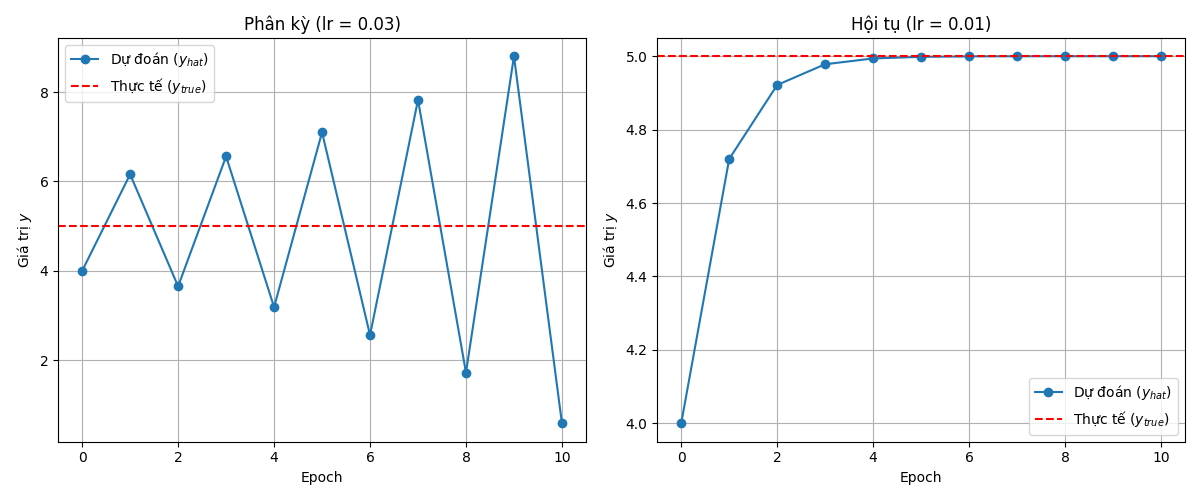
\includegraphics[width=1\linewidth]{img_multiple/diverge_converge.png}
    \caption{Hiện tượng phân kỳ và hội tụ tùy thuộc vào cách chọn tốc độ học}
    \label{fig:diverge_converge}
\end{figure}

\subsection{Quá trình huấn luyện}
\paragraph{Biểu diễn ma trận của mô hình}
Trong mô hình hồi quy tuyến tính đa biến với \( n \) mẫu và \( p \) biến độc lập, ta có thể biểu diễn mô hình dưới dạng ma trận mở rộng để gộp cả tham số bias \( b \) vào:

\begin{itemize}
    \item \( \tilde{X} \in \mathbb{R}^{n \times (p+1)} \): Ma trận dữ liệu mở rộng, với cột đầu tiên là toàn số 1:
    \[
        \tilde{X} = 
        \begin{bmatrix}
            1 & x_{11} & x_{12} & \cdots & x_{1p} \\
            1 & x_{21} & x_{22} & \cdots & x_{2p} \\
            \vdots & \vdots & \vdots & \ddots & \vdots \\
            1 & x_{n1} & x_{n2} & \cdots & x_{np}
        \end{bmatrix}
    \]
    
    \item \( \tilde{\theta} \in \mathbb{R}^{(p+1) \times 1} \): Vector tham số mở rộng, bao gồm cả bias như phần tử đầu tiên:
    \[
        \tilde{\theta} = 
        \begin{bmatrix}
            b \\
            \theta_1 \\
            \theta_2 \\
            \vdots \\
            \theta_p
        \end{bmatrix}
    \]
\end{itemize}

Với cách biểu diễn mở rộng này, mô hình dự đoán có dạng:

\[
    \hat{Y} = \tilde{X}\tilde{\theta}
\]

Trong đó mỗi phần tử \(\hat{y}_i\) của vector \(\hat{Y}\) được tính như sau:

\[
    \hat{y}_i = b + \sum_{j=1}^{p} \theta_j x_{ij}
\]

\paragraph{Đạo hàm ma trận của hàm mất mát}
Hàm mất mát Mean Squared Error (MSE) với cách biểu diễn mở rộng có dạng:

\[
    \mathcal{L}(\tilde{\theta}) = \frac{1}{n} (Y - \tilde{X}\tilde{\theta})^T (Y - \tilde{X}\tilde{\theta})
\]

Gradient của hàm mất mát theo vector tham số mở rộng \(\tilde{\theta}\) là:

\[
    \frac{\partial \mathcal{L}}{\partial \tilde{\theta}} = -\frac{2}{n} \tilde{X}^T(Y - \hat{Y})
\]

Khi phân tích thành các thành phần:

\[
    \frac{\partial \mathcal{L}}{\partial \tilde{\theta}} = -\frac{2}{n} 
    \begin{bmatrix}
        \sum_{i=1}^n (y_i - \hat{y}_i) \\
        \sum_{i=1}^n (y_i - \hat{y}_i)x_{i1} \\
        \sum_{i=1}^n (y_i - \hat{y}_i)x_{i2} \\
        \vdots \\
        \sum_{i=1}^n (y_i - \hat{y}_i)x_{ip}
    \end{bmatrix}
\]

\paragraph{Cập nhật tham số thông qua ma trận}
Sử dụng thuật toán Gradient Descent, ta cập nhật vector tham số mở rộng \(\tilde{\theta}\) như sau:

\[
    \tilde{\theta}^{(t+1)} = \tilde{\theta}^{(t)} + \frac{2\alpha}{n} \tilde{X}^T(Y - \hat{Y}^{(t)})
\]

Cụ thể:

\[
\begin{bmatrix}
    b^{(t+1)} \\
    \theta_1^{(t+1)} \\
    \theta_2^{(t+1)} \\
    \vdots \\
    \theta_p^{(t+1)}
\end{bmatrix} = 
\begin{bmatrix}
    b^{(t)} \\
    \theta_1^{(t)} \\
    \theta_2^{(t)} \\
    \vdots \\
    \theta_p^{(t)}
\end{bmatrix} + 
\frac{2\alpha}{n} 
\begin{bmatrix}
    \sum_{i=1}^n (y_i - \hat{y}_i^{(t)}) \\
    \sum_{i=1}^n (y_i - \hat{y}_i^{(t)})x_{i1} \\
    \sum_{i=1}^n (y_i - \hat{y}_i^{(t)})x_{i2} \\
    \vdots \\
    \sum_{i=1}^n (y_i - \hat{y}_i^{(t)})x_{ip}
\end{bmatrix}
\]

Với \(\alpha\) là tốc độ học và \(t\) là chỉ số của bước lặp trong quá trình huấn luyện.

\subsection{Thử nghiệm mô hình}
Để đảm bảo hiệu năng tối ưu, ta tiến hành thử nghiệm mô hình thông qua nhiều phương pháp huấn luyện khác nhau nhằm xác định cấu hình nào mang lại kết quả tốt nhất.

\subsubsection{Kiến trúc mô hình}
\paragraph{Mô hình cơ sở (base model)}Mô hình cơ sở chính là mô hình tuyến tính đa biến chuẩn mà ta đã thảo luận ở \eqref{eq:mlr}.

\begin{figure}[H]
    \centering
    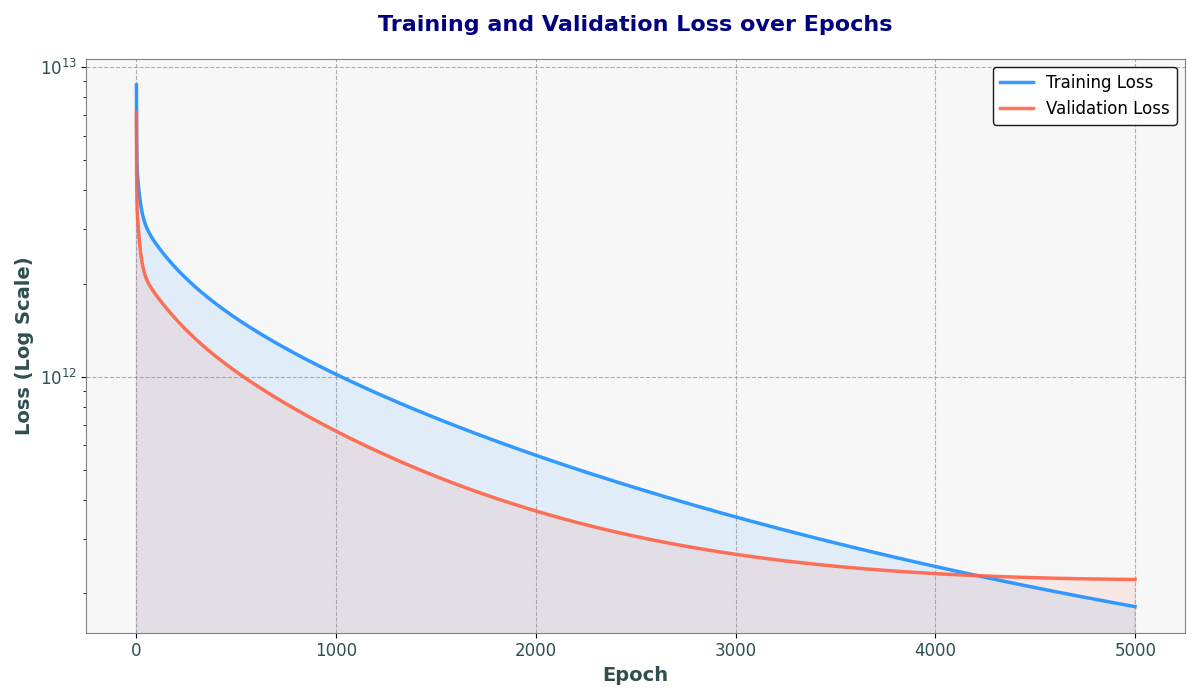
\includegraphics[width=0.9\textwidth]{img_multiple/loss_base.png} % Hình lớn chiếm 90% chiều rộng
    \caption{Giá trị hàm mất mát qua từng epoch (base model)}
    \label{fig:loss_base}
\end{figure}

% Figure 2: Hai subfigure nằm ngang bên dưới
\begin{figure}[H]
    \centering
    \begin{subfigure}[b]{0.48\textwidth}
        \centering
        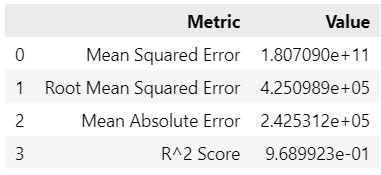
\includegraphics[width=\linewidth]{img_multiple/metrics_base_train.png}
        \caption{Đánh giá trên tập huấn luyện}
    \end{subfigure}
    \hfill
    \begin{subfigure}[b]{0.48\textwidth}
        \centering
        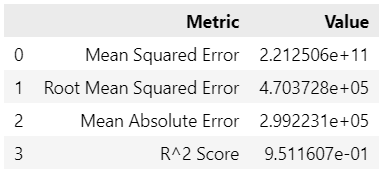
\includegraphics[width=\linewidth]{img_multiple/metrics_base_val.png}
        \caption{Đánh giá trên tập kiểm chứng}
    \end{subfigure}
    \caption{So sánh đánh giá mô hình trên tập huấn luyện và kiểm chứng (base model)} 
\end{figure}

\textit{Nhận xét:} Mô hình cơ sở chưa thông qua các phương pháp gì đặc biệt nhưng vẫn đạt kết quả khá tốt. 

\paragraph{Mô hình không thành phần bias}Theo lý thuyết, việc loại bỏ thành phần bias thường không được khuyến khích vì nó làm giảm đáng kể khả năng biểu diễn và độ phức tạp của mô hình. Để minh họa rõ hơn vấn đề này, ta xét một trường hợp đơn giản với mô hình hồi quy một biến:

\begin{figure}[H]
    \centering
    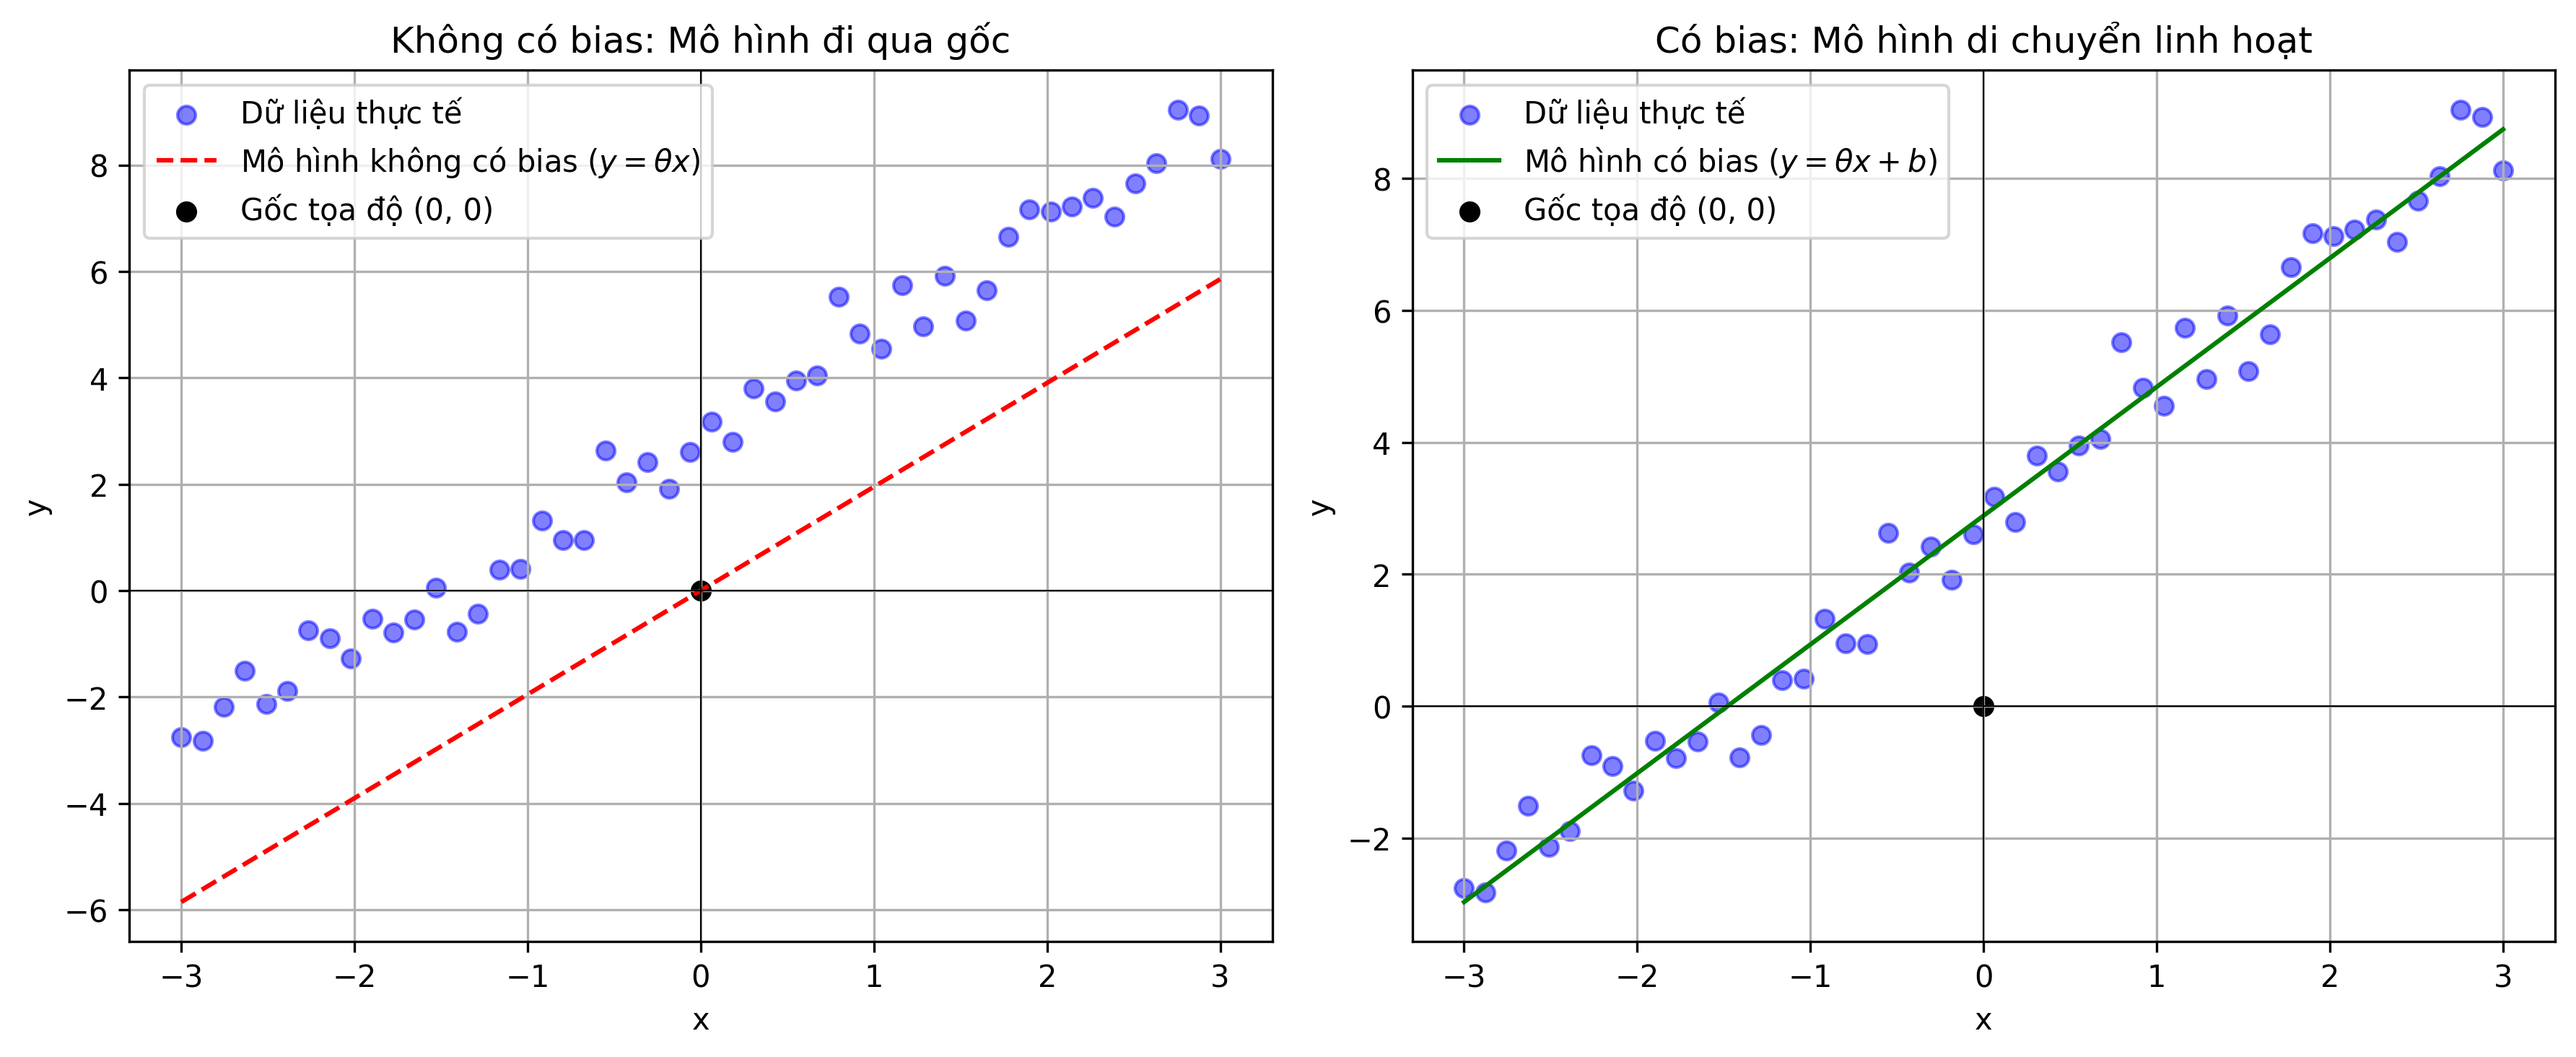
\includegraphics[width=1\linewidth]{img_multiple/bias_comparison_separate.png}
    \caption{So sánh hiệu năng giữa mô hình có và không có thành phần bias}
    \label{fig:bias_comparison}
\end{figure}

Ở mô hình không có bias, mặc dù mô hình học được xu hướng của dữ liệu nhưng do bị giới hạn ở gốc tọa độ, nó không thể nắm bắt được chính xác các mối quan hệ của chúng.

\begin{figure}[H]
    \centering
    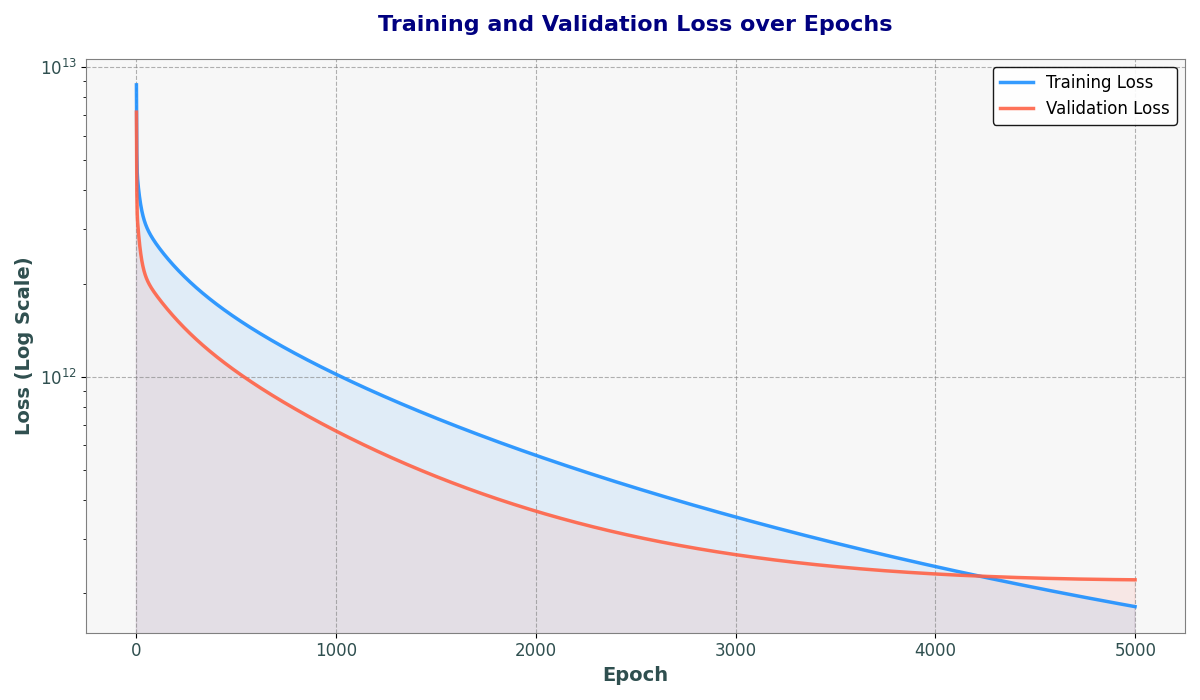
\includegraphics[width=0.9\textwidth]{img_multiple/loss_no_bias.png} % Hình lớn chiếm 90% chiều rộng
    \caption{Giá trị hàm mất mát qua từng epoch (no bias)}
    \label{fig:loss_no_bias}
\end{figure}

% Figure 2: Hai subfigure nằm ngang bên dưới
\begin{figure}[H]
    \centering
    \begin{subfigure}[b]{0.48\textwidth}
        \centering
        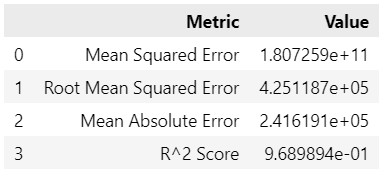
\includegraphics[width=\linewidth]{img_multiple/metrics_no_bias_train.png}
        \caption{Đánh giá trên tập huấn luyện}
    \end{subfigure}
    \hfill
    \begin{subfigure}[b]{0.48\textwidth}
        \centering
        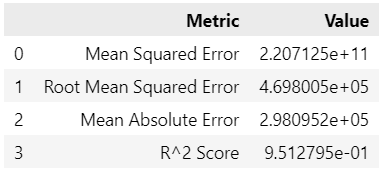
\includegraphics[width=\linewidth]{img_multiple/metrics_no_bias_val.png}
        \caption{Đánh giá trên tập kiểm chứng}
    \end{subfigure}
    \caption{So sánh đánh giá mô hình trên tập huấn luyện và kiểm chứng (no bias)} 
\end{figure}

\subsubsection{Chuyển hóa biến mục tiêu}
Trong các thử nghiệm trước, ta đã sử dụng các đặc trưng đã chuẩn hóa để dự đoán giá nhà ở giá trị gốc. Phần này trình bày các phương pháp chuyển hóa biến mục tiêu nhằm đưa giá trị về phạm vi nhỏ hơn, tạo điều kiện thuận lợi cho quá trình huấn luyện và cải thiện hiệu suất của mô hình.

\paragraph{Phương pháp Min-Max Scaling}
Phép biến đổi Min-Max Scaling được áp dụng theo công thức sau:
\[
    y_{\text{transformed}} = \frac{y_{\text{original}} - y_{\text{min}}}{y_{\text{max}} - y_{\text{min}}}
\]

Phương pháp này chuẩn hóa dữ liệu về khoảng [0, 1], giữ nguyên hình dạng phân phối gốc nhưng thu hẹp phạm vi giá trị.

\begin{figure}[H]
    \centering
    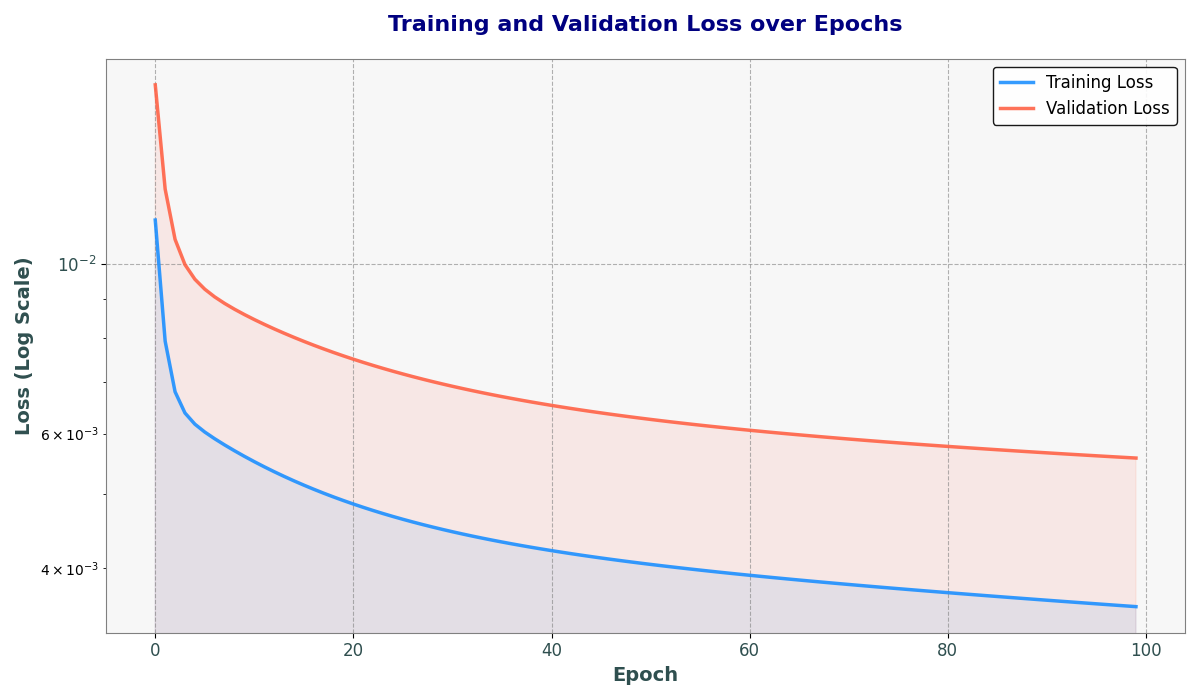
\includegraphics[width=0.9\textwidth]{img_multiple/loss_min_max.png} % Hình lớn chiếm 90% chiều rộng
    \caption{Giá trị hàm mất mát qua từng epoch (Min-Max Scaling)}
    \label{fig:loss_min_max}
\end{figure}

% Figure 2: Hai subfigure nằm ngang bên dưới
\begin{figure}[H]
    \centering
    \begin{subfigure}[b]{0.48\textwidth}
        \centering
        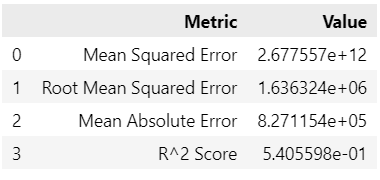
\includegraphics[width=\linewidth]{img_multiple/metrics_min_max_train.png}
        \caption{Đánh giá trên tập huấn luyện}
    \end{subfigure}
    \hfill
    \begin{subfigure}[b]{0.48\textwidth}
        \centering
        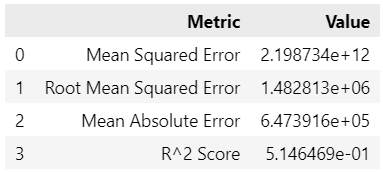
\includegraphics[width=\linewidth]{img_multiple/metrics_min_max_val.png}
        \caption{Đánh giá trên tập kiểm chứng}
    \end{subfigure}
    \caption{So sánh đánh giá mô hình trên tập huấn luyện và kiểm chứng (Min-Max Scaling)} 
\end{figure}

\textit{Nhận xét:} Sau khi chuyển hóa, tốc độ hội tụ của mô hình tăng nhanh đáng kể (chỉ sau khoảng 10 epoch). Hàm mất mát giảm mạnh ở một vài epoch đầu và sườn dốc bắt đầu thoải hơn (giảm chậm) ở các epoch sau chứng tỏ mô hình đã hội tụ.

\paragraph{}{\textbf{Phương pháp chuẩn hóa (Standardization)} \cite{kaggle-standardization}, \cite{youtube-standardization-normalization}: }
Phương pháp chuẩn hóa áp dụng công thức:
\[
    y_{\text{transformed}} = \frac{y_{\text{original}} - \mu_{y}}{\sigma_{y}}
\]

Trong đó $\mu_{y}$ là giá trị trung bình và $\sigma_{y}$ là độ lệch chuẩn của biến mục tiêu. Phương pháp này chuyển đổi dữ liệu về phân phối có trung bình bằng 0 và phương sai bằng 1.

\begin{figure}[H]
    \centering
    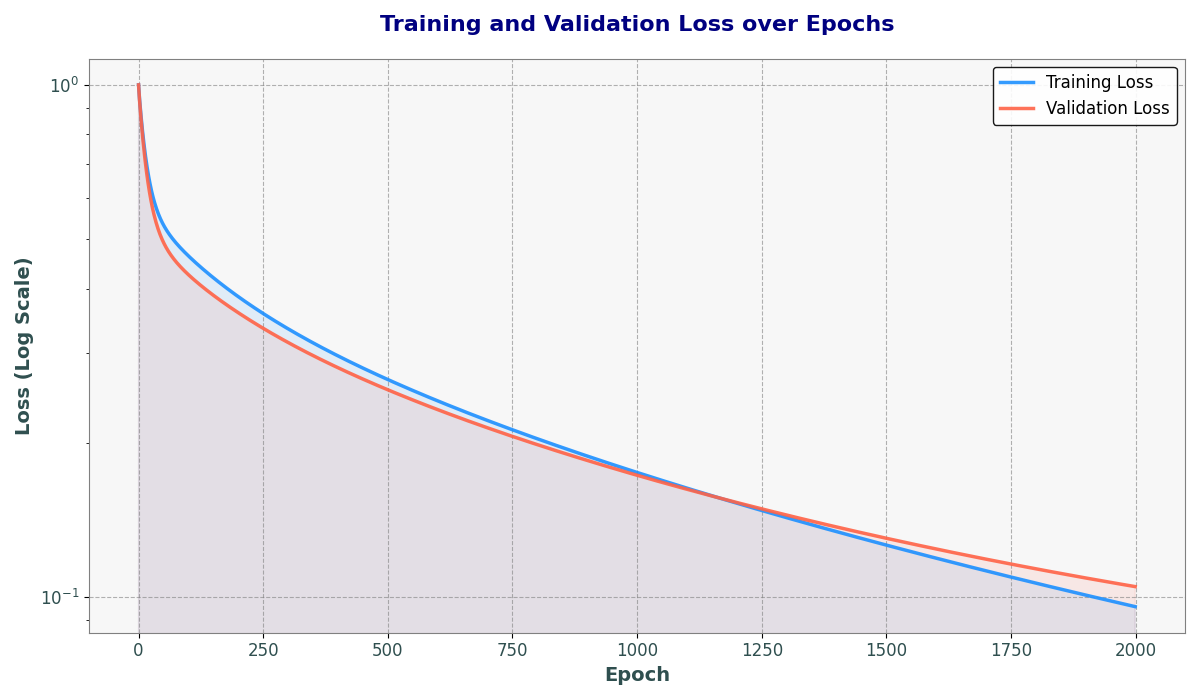
\includegraphics[width=0.9\textwidth]{img_multiple/loss_standardization.png} % Hình lớn chiếm 90% chiều rộng
    \caption{Giá trị hàm mất mát qua từng epoch (Standardization)}
    \label{fig:loss_standardization}
\end{figure}

% Figure 2: Hai subfigure nằm ngang bên dưới
\begin{figure}[H]
    \centering
    \begin{subfigure}[b]{0.48\textwidth}
        \centering
        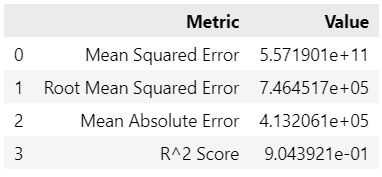
\includegraphics[width=\linewidth]{img_multiple/metrics_standard_train.png}
        \caption{Đánh giá trên tập huấn luyện}
    \end{subfigure}
    \hfill
    \begin{subfigure}[b]{0.48\textwidth}
        \centering
        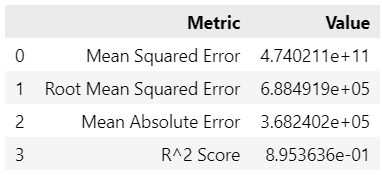
\includegraphics[width=\linewidth]{img_multiple/metrics_standard_val.png}
        \caption{Đánh giá trên tập kiểm chứng}
    \end{subfigure}
    \caption{So sánh đánh giá mô hình trên tập huấn luyện và kiểm chứng (Standardization)} 
\end{figure}

\subsubsection{Regularization}
\paragraph{}{Regularization là phương pháp kiểm soát độ phức tạp của mô hình thông qua việc thêm các ràng buộc vào hàm mục tiêu trong quá trình tối ưu hóa. Phương pháp này đóng vai trò quan trọng trong việc giảm thiểu hiện tượng \textit{quá khớp} (overfitting) trên tập huấn luyện, đồng thời tăng cường khả năng \textit{tổng quát hóa} (generalization) của mô hình. Kết quả là mô hình có thể duy trì độ chính xác cao khi dự đoán trên dữ liệu mới chưa từng được tiếp xúc trong quá trình huấn luyện.}

\paragraph{Hồi quy Lasso (Lasso Regression)}
Phương pháp hồi quy Lasso áp dụng kỹ thuật điều chuẩn L1 thông qua việc bổ sung thành phần phạt vào hàm mất mát, đã được giới thiệu ở \ref{label:lasso-math}.

\begin{figure}[H]
    \centering
    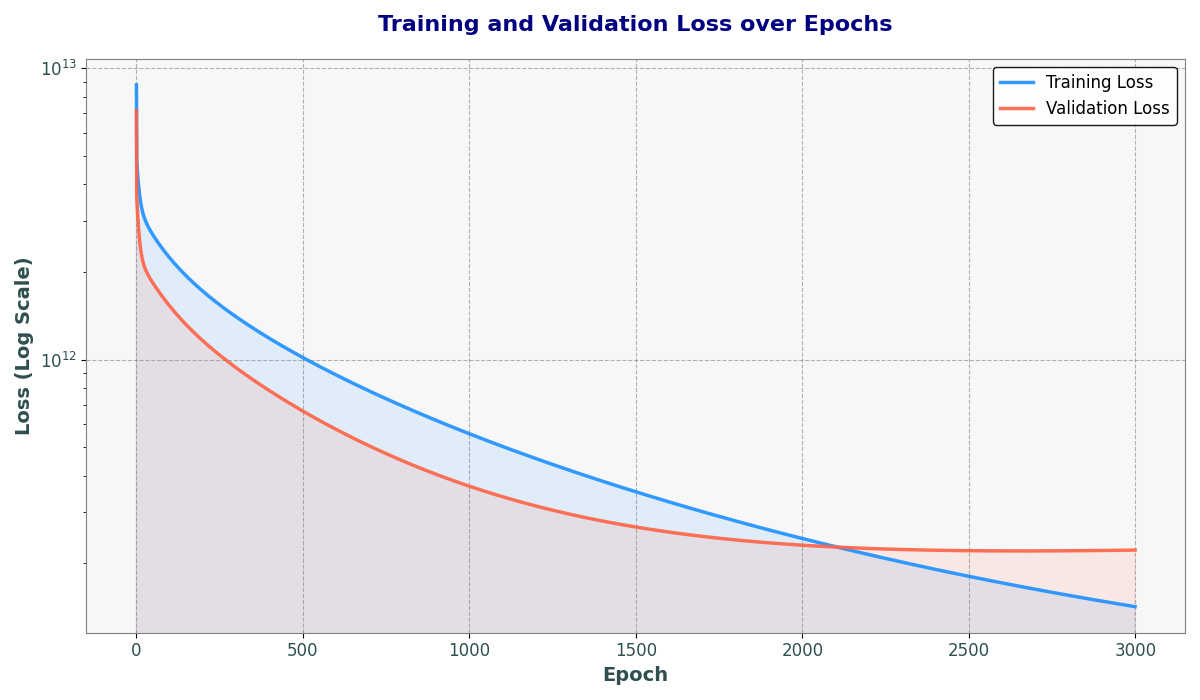
\includegraphics[width=0.9\textwidth]{img_multiple/loss_lasso.png} % Hình lớn chiếm 90% chiều rộng
    \caption{Giá trị hàm mất mát qua từng epoch (Lasso)}
    \label{fig:loss_lasso}
\end{figure}

% Figure 2: Hai subfigure nằm ngang bên dưới
\begin{figure}[H]
    \centering
    \begin{subfigure}[b]{0.48\textwidth}
        \centering
        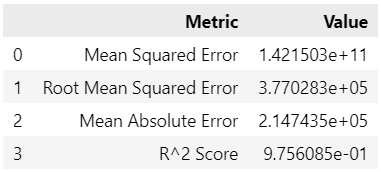
\includegraphics[width=\linewidth]{img_multiple/metrics_lasso_train.png}
        \caption{Đánh giá trên tập huấn luyện}
    \end{subfigure}
    \hfill
    \begin{subfigure}[b]{0.48\textwidth}
        \centering
        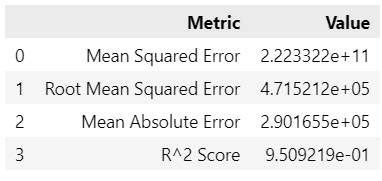
\includegraphics[width=\linewidth]{img_multiple/metrics_lasso_val.png}
        \caption{Đánh giá trên tập kiểm chứng}
    \end{subfigure}
    \caption{So sánh đánh giá mô hình trên tập huấn luyện và kiểm chứng (Lasso)} 
\end{figure}

\paragraph{Hồi quy Ridge (Ridge Regression)}
Phương pháp hồi quy Ridge sử dụng kỹ thuật điều chuẩn L2, đã được giới thiệu ở 2.3.3

\begin{figure}[H]
    \centering
    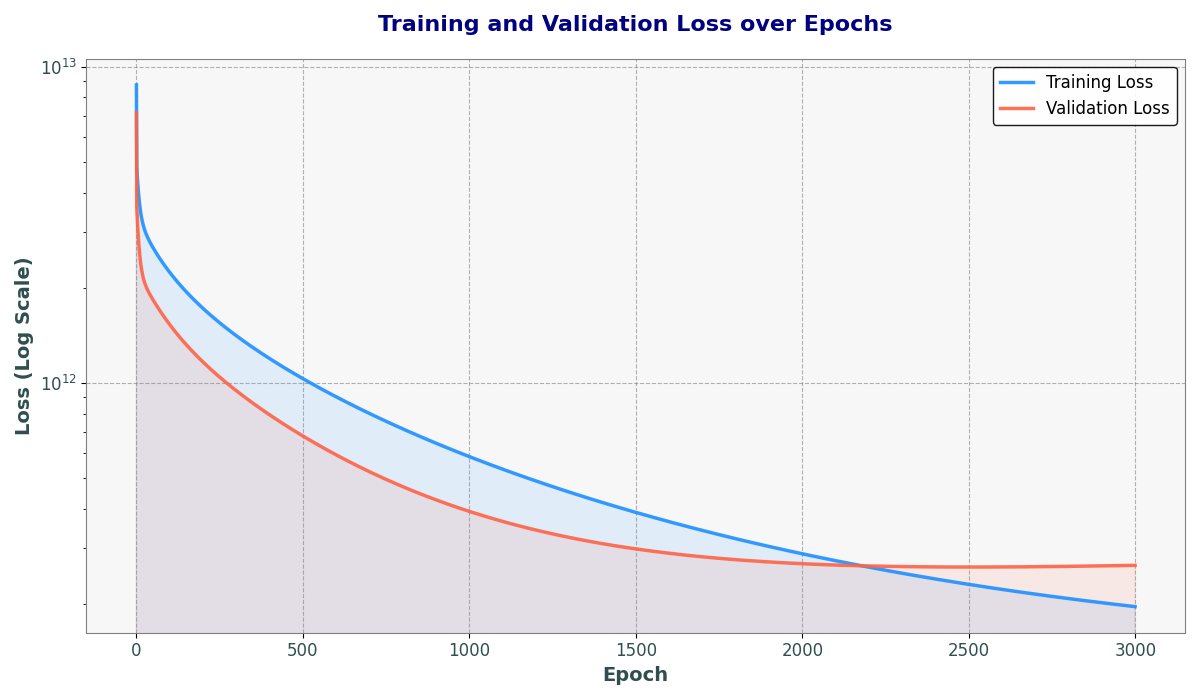
\includegraphics[width=0.9\textwidth]{img_multiple/loss_ridge.png} % Hình lớn chiếm 90% chiều rộng
    \caption{Giá trị hàm mất mát qua từng epoch (Ridge)}
    \label{fig:loss_ridge}
\end{figure}

% Figure 2: Hai subfigure nằm ngang bên dưới
\begin{figure}[H]
    \centering
    \begin{subfigure}[b]{0.48\textwidth}
        \centering
        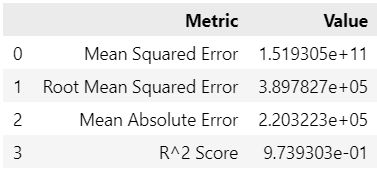
\includegraphics[width=\linewidth]{img_multiple/metrics_ridge_train.png}
        \caption{Đánh giá trên tập huấn luyện}
    \end{subfigure}
    \hfill
    \begin{subfigure}[b]{0.48\textwidth}
        \centering
        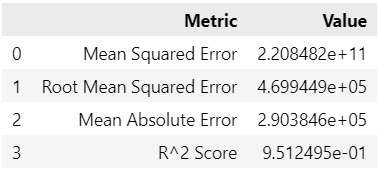
\includegraphics[width=\linewidth]{img_multiple/metrics_ridge_val.png}
        \caption{Đánh giá trên tập kiểm chứng}
    \end{subfigure}
    \caption{So sánh đánh giá mô hình trên tập huấn luyện và kiểm chứng (Ridge)} 
\end{figure}

\subsection{Nhận xét và đánh giá}
\subsubsection{Đánh giá tổng quan hiệu năng mô hình}

Bảng dưới đây trình bày kết quả đánh giá hiệu năng của các mô hình và các phương pháp khác nhau:

\begin{figure}[H]
    \centering
    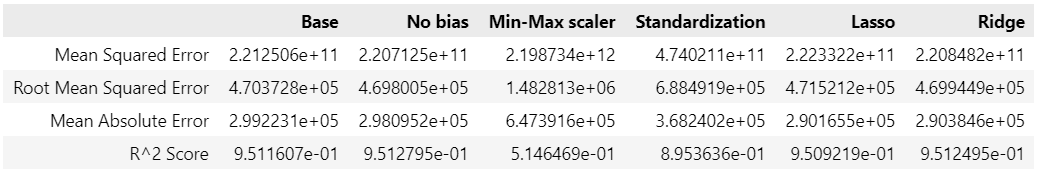
\includegraphics[width=1\linewidth]{img_multiple/summary.png}
    \caption{Tổng kết mức hiệu quả của từng phương pháp}
    \label{fig:summary}
\end{figure}

Phân tích kết quả cho thấy một số điểm đáng chú ý sau:

\begin{enumerate}
    \item \textbf{Về giá trị mất mát:} Các chỉ số MSE (Mean Squared Error) ghi nhận giá trị tương đối cao, lên đến hàng trăm tỷ. Tuy nhiên, điều này không đáng lo ngại vì biến mục tiêu Price vốn có phạm vi giá trị rất lớn. Đặc biệt là với hàm MSE, độ chênh lệch lên cả hàng trăm tỷ vì hàm có bậc bình phương, dẫn đến sẽ đẩy cao giá trị mất mát lên nhiều lần.
    
    \item \textbf{Hiệu suất mô hình cơ sở:} Mô hình cơ sở (Base) và mô hình không thành phần bias (No bias) đều đạt hiệu suất tương đương nhau với chỉ số R$^2$ xấp xỉ 0.951. Điều này cho thấy rằng trong bài toán cụ thể này, thành phần bias không đóng vai trò quan trọng đến hiệu năng của mô hình.
    
    \item \textbf{Tác động của các phương pháp chuyển hóa biến mục tiêu:} Min-Max scaling làm giảm hiệu suất của mô hình đáng kể, với chỉ số R$^2 \approx 0.514$, trong khi đó Standardization đem lại kết quả tương đối tích cực, với R$^2$ đạt gần 0.9
    
    \item \textbf{Hiệu quả của Regularization:} Các phương pháp điều chuẩn (Lasso và Ridge) cho hiệu suất tương đương với mô hình cơ sở (R$^2 \approx 0.951$), chứng tỏ các kỹ thuật regularization có khả năng kiểm soát độ phức tạp của mô hình mà không làm ảnh hưởng đến hiệu suất dự đoán.
\end{enumerate}

\textbf{Kết luận:} Mô hình cơ sở, không bias và các mô hình có áp dụng regularization (Lasso, Ridge) cho hiệu suất xuất sắc với chỉ số R$^2$ đạt 0.951, nghĩa là các mô hình này có khả năng giải thích được 95.1\% phương sai trong dữ liệu giá nhà. Các phương pháp chuyển hóa biến mục tiêu không mang lại cải thiện đáng kể về hiệu suất trong bài toán này, thậm chí còn làm giảm khả năng dự đoán của mô hình.

\subsubsection{Vấn đề với việc chuyển hóa biến mục tiêu}
Tùy thuộc vào bài toán, việc scale biến mục tiêu có thể gia tăng hiệu suất mô hình lên đáng kể (tốc độ học nhanh hơn, tiết kiệm chi phí,...). Theo như thống kê [\ref{fig:summary}], Min-Max scaling đem lại kết quả khá tệ. Lý do có thể là một vài nguyên nhân chính sau đây:

\begin{itemize}
    \item \textbf{Min-Max Scaling}: Phương pháp này đưa biến mục tiêu về khoảng [0,1], giữ nguyên dạng phân phối nhưng nén phạm vi giá trị. Việc nén này có thể làm mất thông tin về không gian giữa các đặc trưng, dẫn đến mô hình học sai các mối quan hệ.

    \begin{figure}[H]
        \centering
        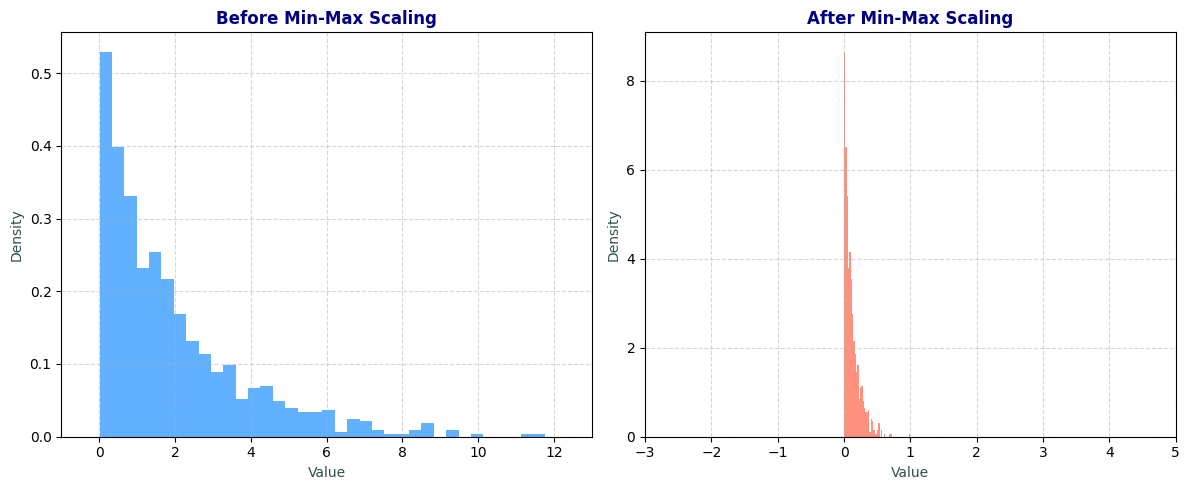
\includegraphics[width=1\linewidth]{img_multiple/output_min_max.png}
        \caption{Minh họa phân phối dữ liệu trước và sau Min-Max Scaling}
    \end{figure}

    \textit{Nhận xét:} Dễ thấy độ phân tán của các điểm dữ liệu thấp do bị ép nén về một phạm vi nhỏ.
    
    \item \textbf{So sánh với Standardization}: Ngược lại, Standardization hoạt động hiệu quả hơn vì đây là một phép biến đổi tuyến tính, nó không làm thay đổi mối quan hệ tuyến tính giữa biến đầu vào và đầu ra, đồng thời, nó vần đưa biến mục tiêu về cùng thang đo với các đặc trưng đã chuẩn hóa, giúp cải thiện hiệu suất.

    \begin{figure}[H]
        \centering
        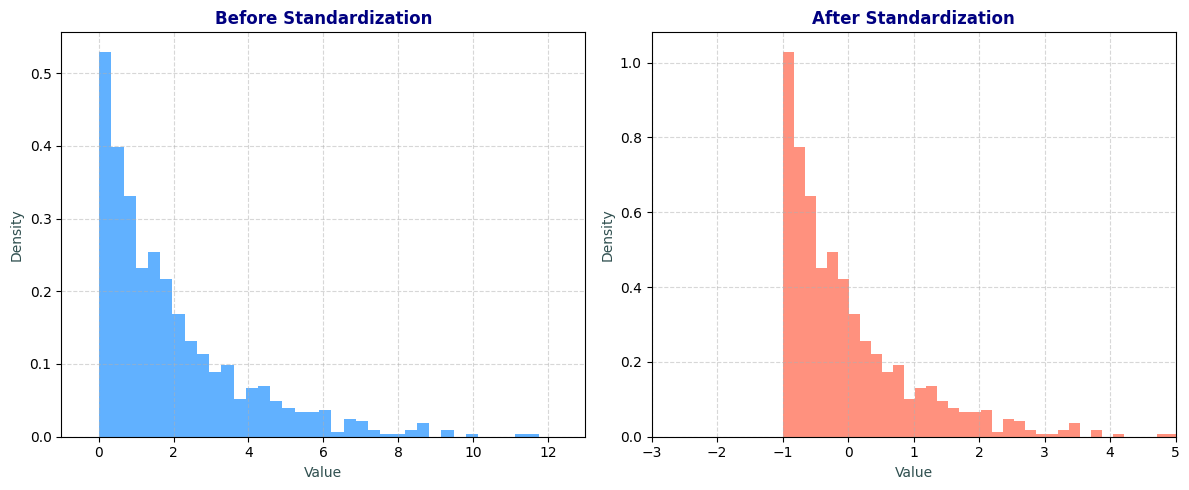
\includegraphics[width=1\linewidth]{img_multiple/output_standard.png}
        \caption{Minh họa phân phối dữ liệu trước và sau Standardization}
    \end{figure}
\end{itemize}

\subsubsection{Kết quả dự đoán của mô hình tốt nhất:}

\begin{figure}[H]
    \centering
    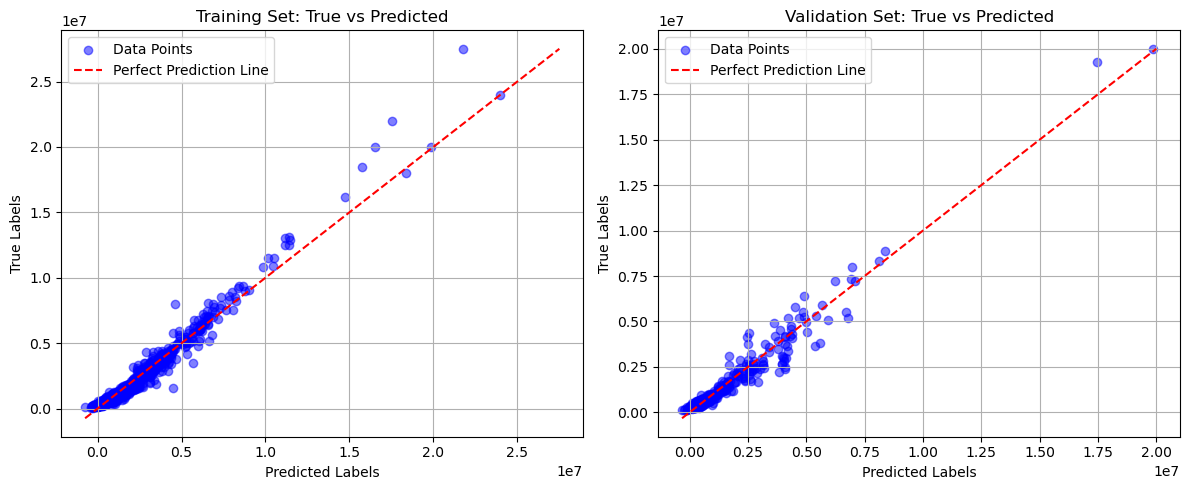
\includegraphics[width=1\linewidth]{img_multiple/output_final.png}
    \caption{Đường thẳng hồi quy dự đoán so với thực tế, trên tập huấn luyện và kiểm chứng}
    \label{fig:enter-label}
\end{figure}

\pagebreak